The Argyris finite element is implemented for each numerical test (described in
\autoref{sec:Tests}). A discussion of Argyris element was presented in
\autoref{sec:FEM}. The Argyris finite element is implemented on an initial mesh
size of $h=\frac{1}{2}$ (\autoref{fig:Mesh}) for each numerical test , and then
the mesh is refined by halving the size of the triangle. The refined results
correspond to a mesh size of $h=\frac{1}{4}$.  This process of mesh refinement
is repeated a total of four times resulting in numerical solutions for mesh
sizes corresponding to
$h=\left\{\frac{1}{2},\frac{1}{4},\frac{1}{8},\frac{1}{16},\frac{1}{32}\right\}$.
\begin{figure}[h]
	\begin{center}
    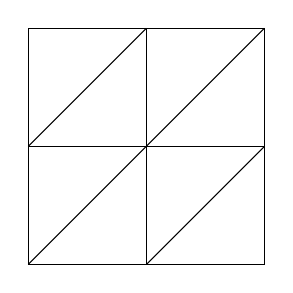
\begin{tikzpicture}[scale=0.5]
\tikzstyle{every node}=[font=\tiny]
      \draw (0,0) -- (6,0) -- (6,6) -- (0,6) -- cycle;
      \draw (0,0) -- (6,6);
      \draw (0,3) -- (6,3);
      \draw (3,0) -- (3,6);
      \draw (0,3) -- (3,6);
      \draw (3,0) -- (6,3);
    \end{tikzpicture}
	\end{center}
  \caption{Initial Mesh with $h=0.5$.}
	\label{fig:Mesh}
\end{figure}


For the numerical tests that are nonlinear, Newton's method is used to solve the
resulting nonlinear system. The stopping criteria for Newton's method is
satisfied when the residue and the two norm of n$^th$ iterate of Newton's method
is less than a given tolerance. If we write Newton's method as
\begin{equation*}
  \Delta_n \psi^h = -\mathcal{J}(\psi^h_{n-1})^{-1}\, F(\psi^h_{n-1}),
\end{equation*}
where $\Delta_n \psi^h = \psi^h_n - \psi^h_{n-1}$ is the n$^th$ iterate of
Newton's method, $\mathcal{J}(\psi^h_{n-1})$ is the Jacobian matrix evaluated at
$\psi^h_{n-1}$, and $F(\psi^h_n-1)$ is the nonlinear problem we are solving
evaluated at $\psi^h_{n-1}$ then the residue, $R$ is given by
\begin{equation*}
  R = \left|F(\psi^h_n)\right|
\end{equation*}
where $|\cdot|$ is the one-norm. In addition to the residue and iterate
conditions for stopping criteria Newton's method is required to terminate if a
max number of iterations is exceeded. For each numerical test the max number of
iterations for Newton's is set to $100$ and the tolerance is set to $10^{-8}$.

After the FE code is run for each $h$, the corresponding $\psi^h$ is used to
calculate the errors $e_0,\, e_1,\text{ and } e_2$, where $e_0,\, e_1,\text{ and
} e_2$ are the $L^2,\, H^1,$ and $H^2$ errors respectively, and are given by
%{\small
\begin{align*}
  e_0 &= \left(\int_{\Omega}\!\left( \psi^h - \psi \right)^2 \,d\vec{x}\right)^{\nicefrac{1}{2}}\\
  e_1 &= \left(e_0^2 + \int_{\Omega}\!  \left( \psi^h_x - \psi_x \right)^2 + \left( \psi^h_y - \psi_y \right)^2
    \,d\vec{x}\right)^{\nicefrac{1}{2}}\\
  e_2 &= \left(e_1^2 + \int_{\Omega}\!  \left( \psi^h_{xx} - \psi_{xx} \right)^2 + \left( \psi^h_{xy} - \psi_{xy}
    \right)^2 + \left( \psi^h_{yy} - \psi_{yy} \right)^2 \,d\vec{x}\right)^{\nicefrac{1}{2}}\\
\end{align*}
%}
The order of convergence, $O$, is then determined by calculating
\begin{equation*}
  O = \dfrac{\log e_{\alpha}^i - \log e_{\alpha}^{i-1}}{\log h_i - \log h_{i-1}},
\end{equation*}
where $e_{\alpha}^i$ is the i$^{th}$ $\alpha$-error corresponding to the
i$^{th}$ mesh size, $h_i$.

Additionally, in each of the convergence data tables we also present the number
of degrees of freedom (DoFs) for Argyris Finite Elements. For the uniform mesh
as described above and a rectangular domain of length, $L$, and height, $H$, the
DoFs are given by
\begin{equation*}
  %DoF = 6\cdot\left(\frac{L}{h}+1\right)\cdot\left(\frac{H}{h}+1\right)+\frac{L}{h}\cdot\left(\frac{H}{h}+1\right)+\left(2\frac{L}{h}+1\right)\cdot\frac{H}{h}.
  N = \frac{7h\left(H + L\right) + 9 H L}{h^2} + 6.
\end{equation*}

